%% 2019 NeuroFedora contributors

%% packages %%
% support for coloured text
\usepackage{xcolor}
\definecolor{FedoraBlue}{cmyk}{1.0,0.46,0.0,0.0}
\definecolor{FedoraDarkBlue}{cmyk}{1.0,0.57,0.0,0.38}
\definecolor{FriendsMagenta}{cmyk}{0.0,0.8,0.4,0.0}
\definecolor{FeaturesOrange}{cmyk}{0.0,0.5,1.0,0.0}
\definecolor{FirstGreen}{cmyk}{0.5,0.0,1.0,0.0}
\definecolor{FreedomPurple}{cmyk}{0.57,0.46,0.0,0.0}

% IPA
\usepackage{tipa}
\usepackage[scale=2]{ccicons}
\usepackage{amssymb}
\usepackage{tikz}
\usetikzlibrary{arrows.meta, arrows, positioning}
\usepackage{jneurosci}
\usepackage{subfig}
\usepackage[T1]{fontenc}
\usepackage[utf8]{inputenc}
\usepackage[style=verbose,backend=biber,autocite=footnote]{biblatex}
\addbibresource{masterbib.bib}
% Use opensans
\usepackage[default,osfigures,scale=0.95]{opensans}
% for strike through
\usepackage[normalem]{ulem}
% links, urls, refs
\usepackage{hyperref}
\hypersetup{colorlinks,linkcolor=FreedomPurple,urlcolor=FreedomPurple}
% graphics
\usepackage{graphicx}
% algorithm
\usepackage{algorithmic}
\usepackage{textcomp}
\usepackage{wrapfig}
\usepackage{textgreek}
\usepackage{euler}
% \usepackage{minted}

% beamer theme
\usetheme[numbering=fraction]{metropolis}
\usefonttheme[onlymath]{serif}
\setbeamerfont{footnote}{size=\tiny}
\setbeamerfont{caption}{size=\tiny}
\setbeamercolor{alerted text}{fg=FeaturesOrange}
\setbeamercolor{progress bar}{fg=FriendsMagenta}
\setbeamercolor{title separator}{fg=FriendsMagenta}
\setbeamercolor{frametitle}{bg=FedoraDarkBlue}

\renewcommand{\figurename}{}

% Not needed in metropolis, but in general footnote citation fixes: https://tex.stackexchange.com/questions/44217/how-can-i-stop-footcite-from-hijacking-my-beamer-columns
% how to use multiple references to the same footnote: https://tex.stackexchange.com/questions/27763/beamer-multiple-references-to-the-same-footnote

%% title %%
\title[NeuroFedora]{\includegraphics[keepaspectratio,width=.25\textwidth]{images/NeuroFedoraLogo01.png}\\NeuroFedora}
\subtitle{FOSS and Free/Open (neuro) Science}
\author{NeuroFedora contributors}
\date[]{}
%% document begins %%
\begin{document}

% title frame %%
\begin{frame}
  \titlepage{}
\end{frame}

%% Three slides for 5 minutes, so 25--30 for 50 minutes.

%% First we define the problem statement. What is it that neuroscience is trying to achieve?
%% Added advantage is that this bit has lots of nice pictures, so it helps to gain the audience's attention.
\section{Problem statement: the brain}
\begin{frame}[c]{The brain: neurons}
  \begin{figure}[h]
    \centering
    \includegraphics[width=\linewidth]{images/Neurons.jpg}
  \end{figure}
  \note[item]{The brain is composed of specialised cells that enable it to process information by the use of electrical impulses}
  \note[item]{As the figure shows, these cells, neurons, have specialised into many many types. They serve different functions, include different proteins and markers, and can be classified in many different ways.}
\end{frame}
\begin{frame}[c]{The brain: in numbers: neurons}
  \begin{columns}
    \begin{column}{0.5\textwidth}
      \begin{figure}[h]
        \centering
        \includegraphics[width=\textwidth]{images/brain-sizes.jpg}
      \end{figure}
    \end{column}
    \begin{column}{0.5\textwidth}
      \begin{itemize}
        \item \alert{86B} neurons\footnotemark{}.
      \end{itemize}
    \end{column}
  \end{columns}
  \vspace{0.2cm}
  \footnotetext[1]{\fullcite{Herculano-Houzel2009}}
  \note[item]{The most recent estimate puts the number of neurons in the human brain at 86B.}
\end{frame}
\begin{frame}[c]{The brain: in numbers: synapses}
  \begin{columns}
    \begin{column}{0.5\textwidth}
      \begin{figure}[h]
        \centering
        \includegraphics[width=\textwidth]{images/reconstruction.jpg}
      \end{figure}
    \end{column}
    \begin{column}{0.5\textwidth}
      \begin{itemize}
        \item \alert{Thousands} of connections between neurons \alert{(synapses)}\footnotemark[2].
        \item Synapses are also of different types, and serve different functions.
          \pause{}
        \item Synapses underlie \alert{learning}\footnotemark[3].
      \end{itemize}
    \end{column}
  \end{columns}
  \vspace{0.2cm}
  \footnotetext[2]{\href{https://drexel.edu/medicine/about/departments/neurobiology-anatomy/research/gao-lab/images/}{Image from The Gao lab, College of Medicine, Drexel University.}}
  \footnotetext[3]{\fullcite{Hebb1949}}
  \note[item]{Each neuron connects with thousands of other neurons, forming a massive network.}
  \note[item]{So, the brain can be thought of as a massively parallel processor.}
\end{frame}
\begin{frame}[c]{So, we want to know (among other things)}
  \begin{itemize}
    \item how the brain functions (\alert{physiology}),
    \item how it is structured (\alert{anatomy}),
    \item about its chemicals (\alert{pharmacology, biochemistry}),
    \item \ldots{}
      \pause{}
    \item how it processes information (\alert{computational}),
    \item about behaviours, and cognition (\alert{behavioural, cognitive}),
    \item \ldots{}
  \end{itemize}
\end{frame}
\begin{frame}[c]{with the aim of applying this knowledge to}
  \begin{itemize}
    \item \alert{disease} prevention and treatment,
    \item \ldots{}
      \pause{}
    \item brain inspired \alert{computing},
    \item \ldots{}
      \pause{}
    \item philosophy and consciousness,
  \end{itemize}
  \note[item]{To take applications from the extreme ends of the spectrum: immediate clinical applications, immediate technological applications.}
\end{frame}
\section{How: research pipeline}
\begin{frame}[c]{General workflow}
  \begin{figure}[h]
    \centering
    \only<1>{\input{images/Neuroscience-cycle}}%
    \only<2>{\input{images/Neuroscience-cycle-complex}}
    \note[item]{A simplified diagram. Actually a lot more complex}
  \end{figure}
\end{frame}
\begin{frame}[c]{Tools of the trade}
  \textcolor{FedoraBlue}{Experimental:}
    \begin{itemize}
      \item EEG, ECoG, intracellular and extracellular single and multi neuron recording,
      \item CT, DOI, MRI, f-MRI, MEG, PET,
    \end{itemize}
    \pause{}
  \textcolor{FriendsMagenta}{Data analysis:}
    \begin{itemize}
      \item Statistics,
      \item Machine Learning, Big Data, Deep learning,
    \end{itemize}
    \pause{}
  \textcolor{FeaturesOrange}{Theory} and \textcolor{FirstGreen}{modelling:}
    \begin{itemize}
      \item Simulators of all kinds, 
    \end{itemize}
  \note[item]{Lots of hardware and software is required for basic neuroscience research.}
\end{frame}
\begin{frame}[c]{Tools of the trade:\ II}
  \textcolor{FedoraDarkBlue}{Tools for the dissemination of knowledge\footnotemark[4]:}
  \begin{itemize}
    \item visualisation,
    \item academic writing,
    \item non academic writing: blogging \ldots,
    \item podcasting,
    \item video making,
    \item creating teaching materials,
  \end{itemize}
  \pause{}
  \textcolor{FirstGreen}{Collaborative tools and utilities.}
  \footnotetext[4]{also to a non-specialist audience.}
  \note[item]{Often ignored, but not less important}
\end{frame}
\section{Free/Open (neuro) Science?}
\begin{frame}[c]{A familiar ideal}
  Free/Open science:\\\alert{Everyone} should have the freedom to \alert{share, study, and modify} scientific material.\\
  \note[item]{This includes all research related activities, tools, and output, not only source code.}
  \pause{}
  \vspace{0.5cm}
  FOSS\@:\\\alert{Everyone} should have the freedom to \alert{share, study, and modify} software\footnotemark[5].\\
  \pause{}
  \vspace{0.5cm}
  \alert{Free/Open Science implicitly includes, and relies heavily on FOSS.}\\
  \footnotetext[5]{\href{https://u.fsf.org/user-liberation}{Free software foundation}}
\end{frame}
\begin{frame}[c]{Now,}
  \alert{FOSS is becoming the standard in research\footnotemark[6].}
  \begin{figure}[htpb]
    \centering
    \includegraphics[width=\linewidth]{images/open-source-paper.png}
  \end{figure}
  \footnotetext[6]{\href{http://opensourceforneuroscience.org/}{Open source for neuroscience}}
\end{frame}
\section{What can we, Fedora, do to help?}
\begin{frame}[c]{Neuroscience community: highly multidisciplinary}
  \begin{itemize}
    \item \alert{various specialities:} biologists, mathematicians, physicists, chemists, psychologists, \ldots, 
      \pause{}
    \item \alert{small proportion of trained software developers},
  \end{itemize}
\end{frame}
\begin{frame}[c]{(Anecdotal) notes on development of research software}
  \begin{itemize}
    \item often \alert{single developer}, or small development teams,
      \pause{}
    \item limited \alert{access to hardware/resources},
      \pause{}
    \item limited \alert{code quality},
      \pause{}
    \item limited \alert{use of established best practices},
      \pause{}
    \item limited \alert{testing for correctness (!)},
      \pause{}
    \item limited \alert{maintenance, short-lived projects},
      \pause{}
    \item \alert{complex dependency chains},
      \pause{}
    \item lack of \alert{documentation and support},
      \pause{}
    \item lack of \alert{community development know-how},
  \end{itemize}
  \note[item]{Give how interdisciplinary neuroscience is, most researchers are NOT trained in development}
  \note[item]{This implies, and this is based on anecdotal evidence, that the software used in research is not of the best quality}
\end{frame}
\begin{frame}[c]{(Anecdotal) notes on users of research software}
  \begin{itemize}
    \item \alert{waste time and effort} installing (and reinstalling) their software stacks,
      \pause{}
    \item are \alert{unaware of helpful development tools},
      \pause{}
    \item \alert{rarely run test suites (!)},
      \pause{}
    \item \alert{rarely report bugs} upstream,
      \pause{}
    \item \alert{rarely send improvements} upstream,
  \end{itemize}
  \note[item]{The other side of the bridge is the users}
  \note[item]{Because they aren't trained, they have a hard time setting up and using the software}
  \note[item]{If correctness of a tool cannot be verified, how can the correctness of the scientific result be claimed?}
\end{frame}
\begin{frame}[c]{We, at Fedora, are in a unique position}
  \begin{itemize}
    \item we \alert{liaison between upstream and users} already,
      \pause{}
    \item we \alert{follow best practices} in software development,
      \pause{}
    \item we have the \alert{infrastructure},
      \pause{}
    \item we constantly \alert{work to grow the community},
      \pause{}
    \item we \alert{learn from one another}---train as we work,
      \pause{}
    \item we \alert{disseminate} information to end-users,
  \end{itemize}
\end{frame}
\begin{frame}[c]{So, we started NeuroFedora}
  \textcolor{FedoraBlue}{Primary goal:}
  \begin{itemize}
    \item Provide a \alert{ready to use, integrated FOSS platform} for neuroscientists\footnotemark[7].
  \end{itemize}
  \pause{}
  \textcolor{FirstGreen}{Secondary/collateral goals:}
  \pause{}
  \begin{itemize}
    \item help \alert{improve the standard and maintenance} of tools,
    \item help users \alert{develop software development skills},
    \item \alert{make neuroscience accessible} to non-specialists,
      \pause{}
    \item \textcolor{FriendsMagenta}{make Fedora the go-to distribution for neuroscience}.
  \end{itemize}
  \footnotetext[7]{Researchers, academics, hobbyists, anyone!}
\end{frame}
\begin{frame}[c]{In essence,}
  \textcolor{FedoraBlue}{NeuroFedora is:\\}
  \begin{itemize}
    \item \textcolor{FriendsMagenta}{merely leveraging pre-existing community resources to a new domain of software.}\\
      \pause{}
    \item \textcolor{FeaturesOrange}{taking the community model of FOSS to neuroscience research,}
  \end{itemize}
\end{frame}
\begin{frame}[c]{NeuroFedora: current metrics}
  \begin{itemize}
    \item \alert{less than a year old\footnotemark[8],}
      \pause{}
    \item \textcolor{FirstGreen}{15 active contributors:}
      \begin{itemize}
        \item 10 package maintainers,
        \item 5 designers, newcomers,
        \item only 5 from a neuroscience background,
      \end{itemize}
      \pause{}
    \item \textcolor{FriendsMagenta}{software:}
      \begin{itemize}
        \item 105 packages ready to install\footnotemark[9].
        \item \textasciitilde{}160 in queue\footnotemark[10].
      \end{itemize}
      \pause{}
    \item \textcolor{FedoraBlue}{poster presented at annual Computational Neuroscience Conference (CNS), 2019\footnotemark[11].}
  \end{itemize}
  \footnotetext[8]{in its second iteration}
  \footnotetext[9]{\href{https://src.fedoraproject.org/group/neuro-sig}{src.fedoraproject.org: Neuro-SIG}}
  \footnotetext[10]{\href{https://pagure.io/neuro-sig/NeuroFedora/issues?status=Open&tags=T\%3A+Software}{Pagure.io: Neuro-SIG: issues}}
  \footnotetext[11]{\href{https://neurofedora.github.io/2019/07/11/neurofedora-poster-at-cns-2019.html}{NeuroFedora blog: poster at CNS*2019}}
\end{frame}
\begin{frame}[c]{NeuroFedora: future plans}
  \begin{itemize}
    \item \alert{make more software available,}
      \begin{itemize}
        \item \alert{via modularity,}
        \item \alert{via containers,}
      \end{itemize}
      \pause{}
    \item \textcolor{FirstGreen}{improve documentation, and support,}
      \pause{}
    \item \textcolor{FriendsMagenta}{increase community,}
      \begin{itemize}
        \item \textcolor{FriendsMagenta}{convert research user base into FOSS contributors,}
        \item \textcolor{FriendsMagenta}{convert FOSS contributor base into users,}
      \end{itemize}
  \end{itemize}
\end{frame}
\begin{frame}[c]{NeuroFedora: what you can do}
  \textcolor{FriendsMagenta}{Anything! It's just more of Fedora!}
  \pause{}
  \begin{columns}
    \begin{column}{0.5\textwidth}
      \begin{itemize}
        \item packaging,
        \item testing
        \item containers,
        \item documentation,
        \item evangelism,
        \item marketing,
        \item design,
        \item \ldots,
      \end{itemize}
    \end{column}
    \begin{column}{0.5\textwidth}
      \begin{figure}[h]
        \centering
        \includegraphics[width=0.8\linewidth]{images/NeuroFedoraBadge.png}
      \end{figure}
    \end{column}
  \end{columns}
\end{frame}
\section{So!}
\begin{frame}[c]{There's so much more to talk about}
  \textcolor{FedoraBlue}{Mailing list:\ neuro-sig@lists.fedoraproject.org}\\
  \textcolor{FirstGreen}{IRC:\ \#fedora-neuro}\\
  \textcolor{FeaturesOrange}{Telegram:\ t.me/NeuroFedora}\\
  \textcolor{FriendsMagenta}{Docs:\ neuro.fedoraproject.org}\\
  \textcolor{FirstGreen}{Blog:\ neurofedora.github.io}\\
  \textcolor{FeaturesOrange}{Pagure:\ neuro-sig/NeuroFedora}
\end{frame}
\begin{frame}[c]{Fedora \ensuremath\heartsuit{} Science}
  \textcolor{FreedomPurple}{There's more science in Fedora! Come to the HACKATHON!}
  \begin{itemize}
    \item \textcolor{FedoraBlue}{Astronomy SIG}
    \item \textcolor{FirstGreen}{Bigdata SIG}
    \item \textcolor{FeaturesOrange}{Machine Learning}
    \item \textcolor{FriendsMagenta}{Electronic Lab}
    \item \textcolor{FedoraBlue}{Medical}
    \item \textcolor{FirstGreen}{Sci-tech}
  \end{itemize}
  \pause{}
  \textcolor{FreedomPurple}{Is your interest not listed? Start your own!}
  \note[item]{All the resources are already available in the community---all one needs to do is find others who share interests and start working!}
\end{frame}
% If time permits, and the audience looks interested
\section{Myths}
\begin{frame}[c]{Myth 1}
  \textcolor{FriendsMagenta}{(Neuro) science is all about working on \enquote{core research}.}\\
  \vspace{0.5cm}
  \pause{}
  \textcolor{FirstGreen}{Wrong! There is more to (neuro) science!}\\
  \note[item]{The learning curve is similar to what non-techies experience when they try to join FOSS\@. It takes similar effort to gain the required domain specific knowledge.}
\end{frame}
\begin{frame}[c]{Myth buster example: Open Source Brain}
  \begin{figure}[h]
    \centering
    \includegraphics[width=\linewidth]{images/OSB.png}
  \end{figure}
  \footnotetext[12]{\href{https://opensourcebrain.org}{opensourcebrain.org}}
\end{frame}
\begin{frame}[c]{Myth buster example: OpenWorm }
  \begin{figure}[h]
    \centering
    \includegraphics[width=\linewidth]{images/openworm.png}
  \end{figure}
  \footnotetext[13]{\href{https://openworm.org}{openworm.org}}
\end{frame}
\begin{frame}[c]{Myth buster example: Science art}
  \begin{columns}
    \begin{column}{0.5\textwidth}
      \begin{figure}[h]
        \centering
        \includegraphics[height=0.6\textheight]{images/rebeccaivatts-dementia.jpg}
        \caption{Snail: related to Dementia}
      \end{figure}
    \end{column}
    \begin{column}{0.5\textwidth}
      \begin{figure}[h]
        \centering
        \includegraphics[height=0.6\textheight]{images/rebeccaivatts-pieces-of-mind.jpg}
        \caption{Pieces of the Mind (2014)}
      \end{figure}
    \end{column}
  \end{columns}
  \footnotetext[14]{\href{https://rebeccaivatts.com}{rebeccaivatts.com}, \textcopyright{} Rebecca Ivatts 2019}
\end{frame}
\begin{frame}[c]{Myth 2}
  \textcolor{FriendsMagenta}{Only researchers can do (neuro) science. It's too hard.}\\
  \vspace{0.5cm}
  \pause{}
  \textcolor{FirstGreen}{Wrong! Everyone can do (neuro) science!}\\
  \note[item]{The learning curve is similar to what non-techies experience when they try to join FOSS\@. It takes similar effort to gain the required domain specific knowledge.}
\end{frame}
\begin{frame}[c]{Myth buster example: understanding learning}
  \note[item]{We learn when synapses change in the brain}
  \note[item]{As an example, let's say we have a neuron that was activated by a smell.}
  \note[item]{Later, we found out that that was the smell of some food, say curry.}
  \note[item]{Because these neurons fired one after the other here, this synapse is strengthened.}
  \note[item]{When this happens repeatedly, the synapse is strengthened again and again.}
  \note[item]{Until, the faintest whiff of the smell reminds you of the food!}
  \begin{columns}
    \begin{column}{0.5\textwidth}
      \begin{figure}[h]
        \centering
        \only<1>{\input{images/ltp-schematic-1.tex}}
        \only<2>{\input{images/ltp-schematic-2.tex}}
        \only<3>{\input{images/ltp-schematic-3.tex}}
        \only<4>{\input{images/ltp-schematic-4.tex}}
        \only<5>{\input{images/ltp-schematic-5.tex}}
      \end{figure}
    \end{column}
    \begin{column}{0.5\textwidth}
      \begin{figure}[h]
        \centering
        \def\lenspike{0.5cm}
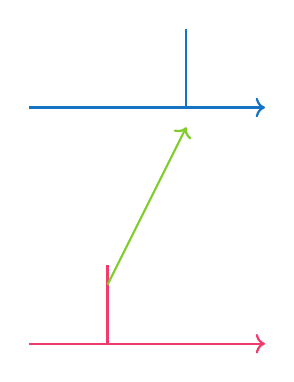
\begin{tikzpicture}[scale=1, transform shape]
  % Neuron 1
  \def\circlex{0}
  \def\circley{0}
  \draw [FriendsMagenta, thick, ->] (\circlex, \circley) -- ++ (3cm, 0);
  \draw [FriendsMagenta, thick] (\circlex + 1cm, \circley) -- ++ (0, \lenspike);

  \draw [FirstGreen, thick, ->] (\circlex + 1cm, \circley + 0.75) -- ++ (\circlex + 1cm, 2);

  % Neuron 2
  \def\circlex{0}
  \def\circley{3}
  \draw [FedoraBlue, thick, ->] (\circlex, \circley) -- ++ (3cm, 0);
  \draw [FedoraBlue, thick] (\circlex + 2cm, \circley) -- ++ (0, \lenspike);


\end{tikzpicture}



      \end{figure}
    \end{column}
  \end{columns}
  \footnotetext[15]{Spike-timing dependent plasticity (STDP): underlies learning in the Brain.}
  \note[item]{Of course, the more you look at it, the more information you find, but that doesn't mean that we can't study or apply it.}
\end{frame}
\begin{frame}[fragile]{Myth buster example: an example simulation in NEST}
  \tiny{
  \begin{verbatim}
# sudo dnf install python3-nest
import pylab
import nest
import nest.voltage_trace

weight = 20.0
delay = 1.0
stim = 1000.0

# create two neurons and a voltmeter
neuron1 = nest.Create("iaf_psc_alpha")
neuron2 = nest.Create("iaf_psc_alpha")
voltmeter = nest.Create("voltmeter")

# give the first neuron a stimulus, connect it to the second one, watch the second spike
nest.SetStatus(neuron1, {"I_e": stim})
nest.Connect(neuron1, neuron2, syn_spec={'weight': weight, 'delay': delay})
nest.Connect(voltmeter, neuron2)

nest.Simulate(100.0)

nest.voltage_trace.from_device(voltmeter)
nest.voltage_trace.show()
  \end{verbatim}
}

  \note[item]{This is all it takes to simulate two neurons that are connected through a synapse.}
  \note[item]{Of course, this is a simple example, but the point is---it's just programming with a little bit of domain knowledge.}
  \footnotetext[16]{\href{https://nest-simulator.org}{nest-simulator.org}}
\end{frame}
\end{document}
